\section{Results}
	\subsection{Descriptive Analysis}

	\subsection{ARIMA model}
	\paragraph{Time series decomposition}The time series of total dengue cases in Thailand was additively decomposed in the components trend, seasonal and random, as shown in Figure \ref{fig:decomp_ts_dengue}. The time series shows a seasonal pattern with a frequency of 12 months. The trend shows fluctuation over the time period with two periods of comparatively high dengue cases in 2013/14 and 2015/16.
	
	\begin{figure}[htbp] 
		\centering
		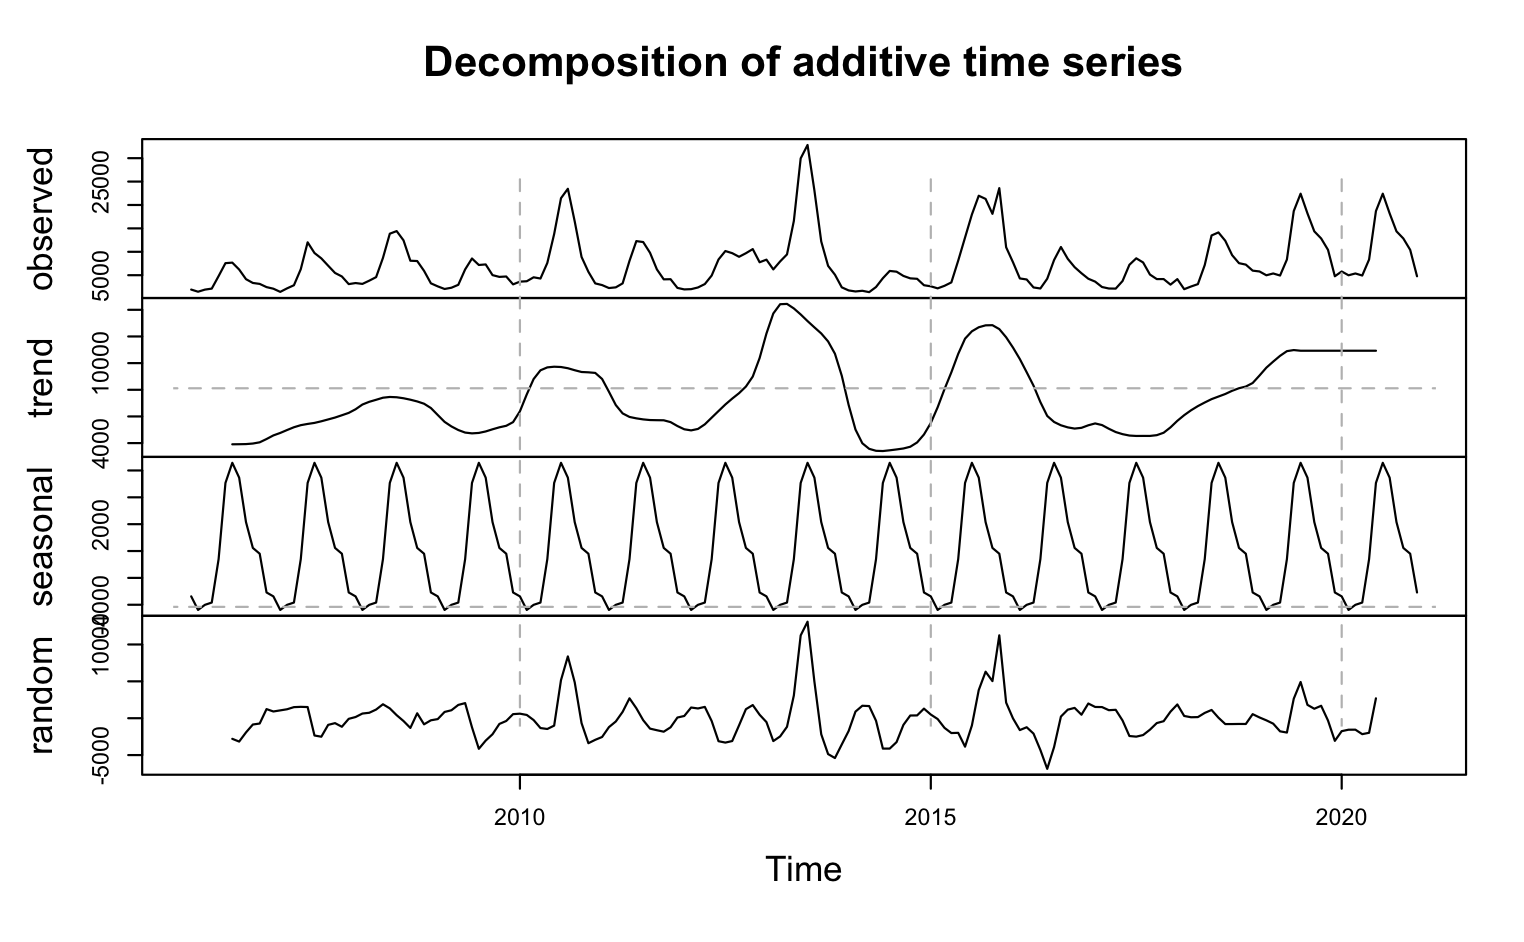
\includegraphics[width=0.7\textwidth]{fig/Decomposition_of_add_ts.png}
		\caption{ Decomposition of the additive time series of the total dengue cases in Thailand}
		\label{fig:decomp_ts_dengue}
	\end{figure}
	
	The decomposition of the time series of the dengue cases was compared to the decomposition of the time series of temperatures. Both time series have an annual seasonal pattern. The trends show in general similar patterns with differences in the amplitudes and slight shifts on the time axis, as shown in Figure \ref{fig:Trend_temp_cases}.
	\begin{figure}[hbpt] 
		\centering
		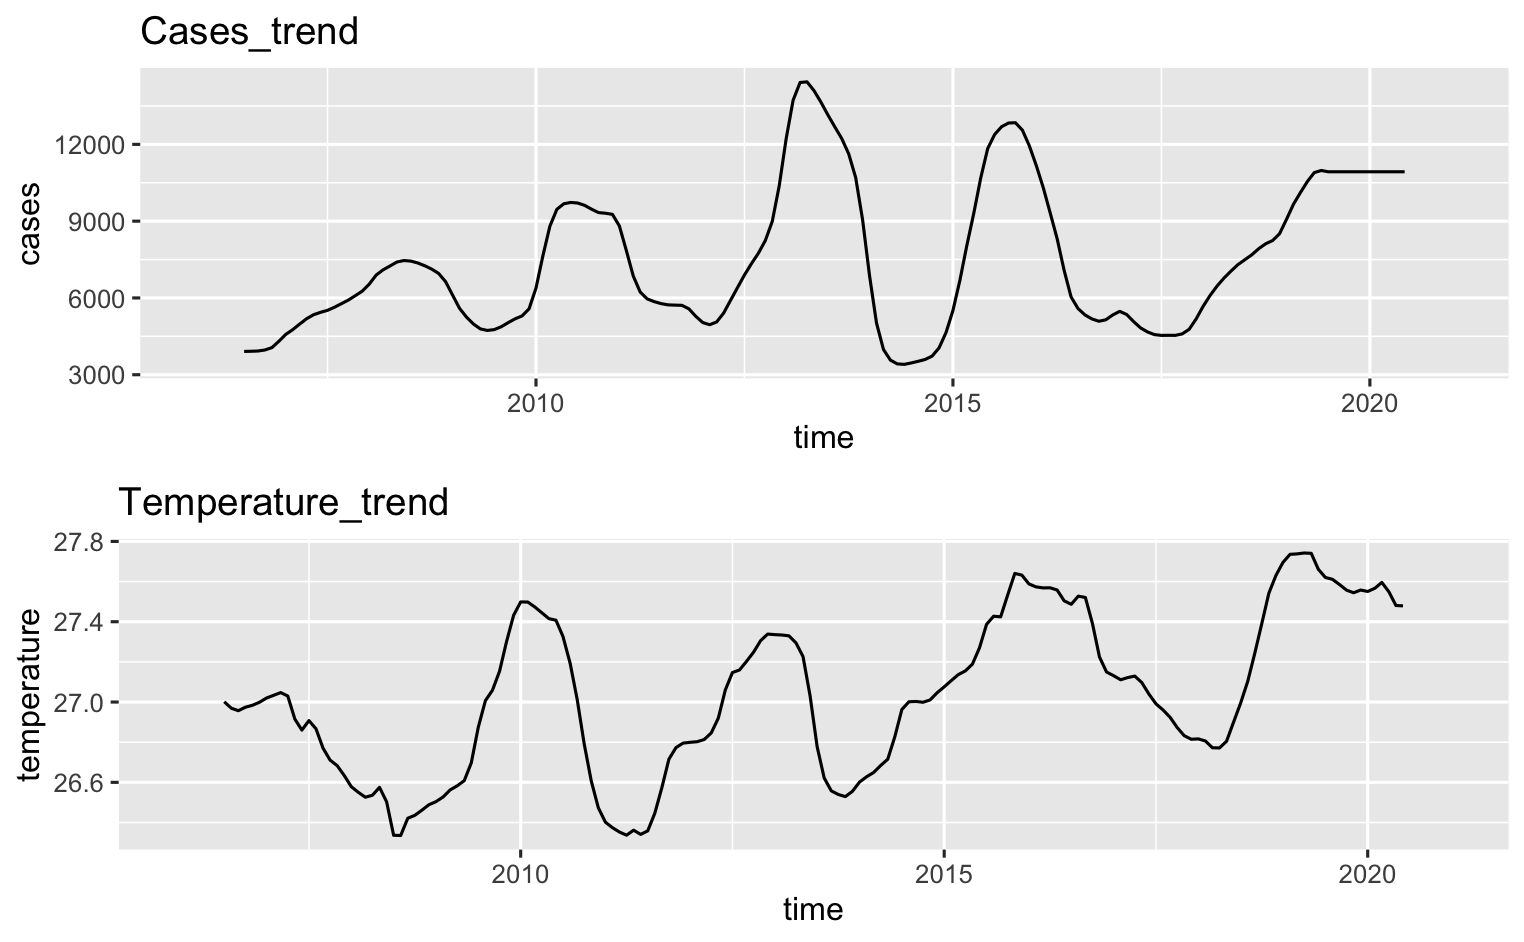
\includegraphics[width=0.7\textwidth]{fig/Trend_temp_cases.png}
		\caption{Trend of the total dengue cases in Thailand compared to the trend of the average temperature in Thailand for the years 2006 till 2020.}
		\label{fig:Trend_temp_cases}
	\end{figure}
	 In 2010 and 2012/13, there were temperature peaks, followed by peaking dengue cases a few months after. In 2015/16 rising temperatures were accompanied by rising dengue cases. 
	\paragraph{ARIMA forecast}
	
	ARIMA modeling was performed to forecast the dengue case development in Thailand. For ADF test results, a p-value of 0.01 was used, for the KPSS test results a p-value of 0.1 was used. Therefore both test indicate stationarity of the time series and differencing isn’t necessary. Observation of the time series ACF showed oscillations which suggests the presence of seasonality in the data. The pACF exhibits a notable pattern with an initial positive peak followed by a significant negative peak. This pattern indicates the need to consider both autoregressive and moving average components in the model.
	To test for the optimal ARIMA model, models with different combinations of p, d and q values were generated and the best model was selected by comparing the AICs. The best model was found to be (2,2,2) with an AIC of 3319.732. Because this method could not account for seasonality in the data, the auto.arima function was used. “ARIMA(1,0,2)(1,1,0)[12] with drift” was found to be the best model. This model consists of an autoregressive term and two moving average terms. No differencing was performed. The model also has seasonal compounds with a period of 12. “With drift” means that a constant is included in the model. As the AIC of 3108.35 is lower and thus more accurate than the AIC of the former model, the auto.arima model was used for further analysis. 
	The evaluation of the histogram of the residuals revealed that the residuals were distributed similar to a normal distribution. The ACF plot indicates some significant autocorrelation at lag 1, while the remaining lags show no significant autocorrelation. The p-value of the Ljung-Box test was 0.41. Thus, the residuals are not distinguishable from white noise and the model has adequately captured the information in the data. 
	Based on the model, a forecast was made for the next four years, which extends beyond the data (see Figure \ref{fig:Auto_ARIMA_forecast}). 
	
		\begin{figure}[hbpt] 
		\centering
		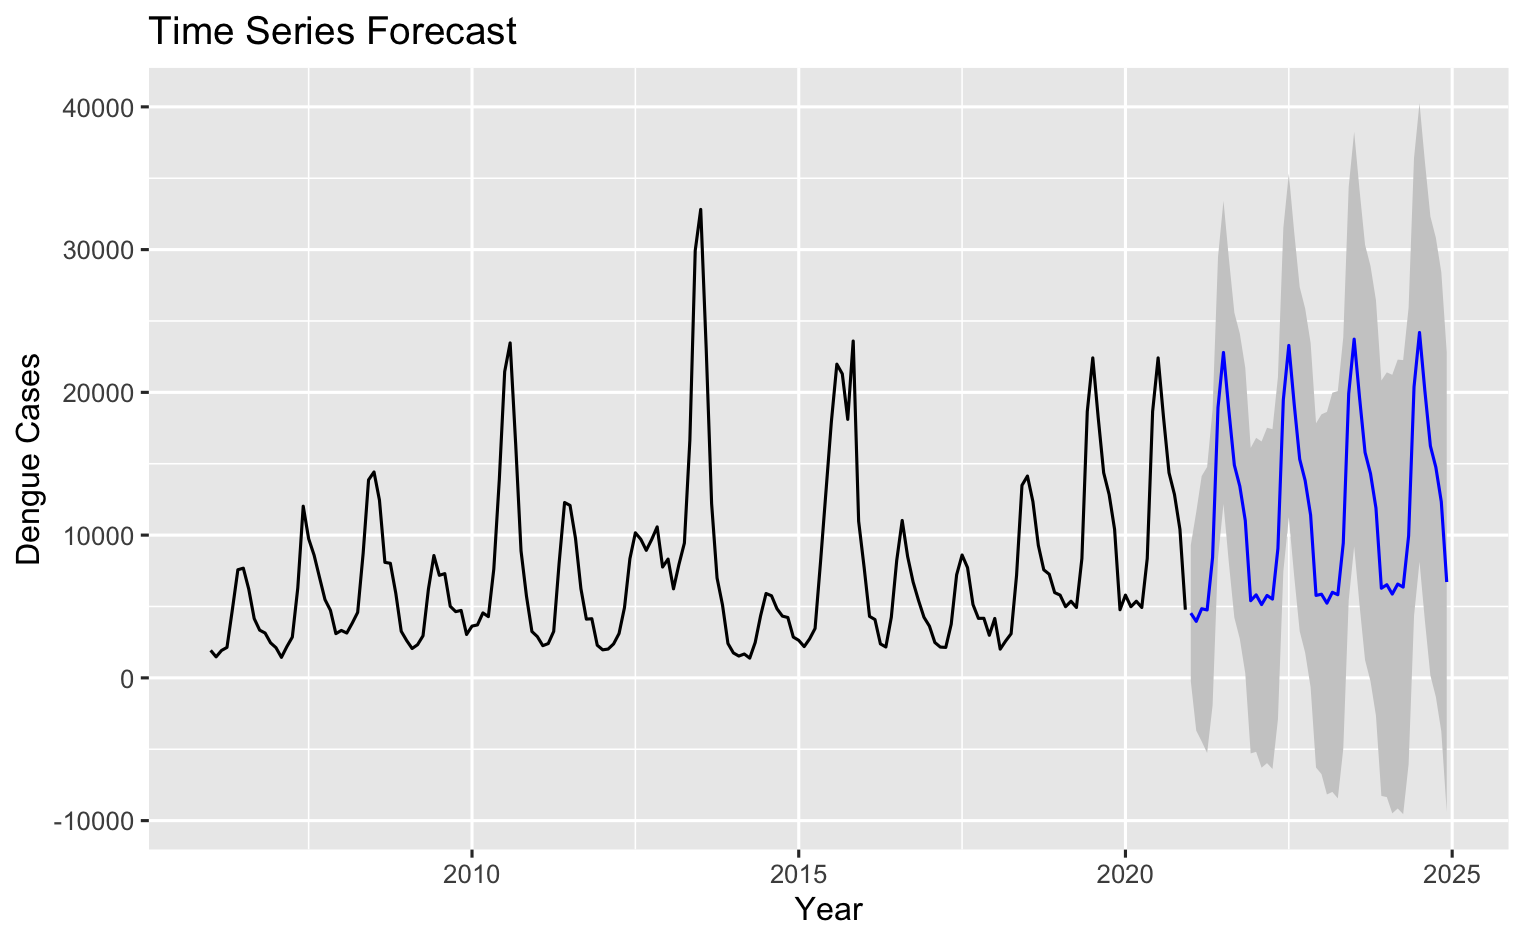
\includegraphics[width=0.7\textwidth]{fig/Auto_ARIMA_forecast.png}
		\caption{ARIMA forecast of the dengue cases in Thailand for 2021-2024.}
		\label{fig:Auto_ARIMA_forecast}
	\end{figure}
 
	To compare the accuracy of the forecast, the time series was cropped after December 2016 and the years 2017 till 2020 were forecasted, as shown in Figure \ref{fig:Auto_ARIMA_2016}. 
		\begin{figure}[hbpt] 
		\centering
		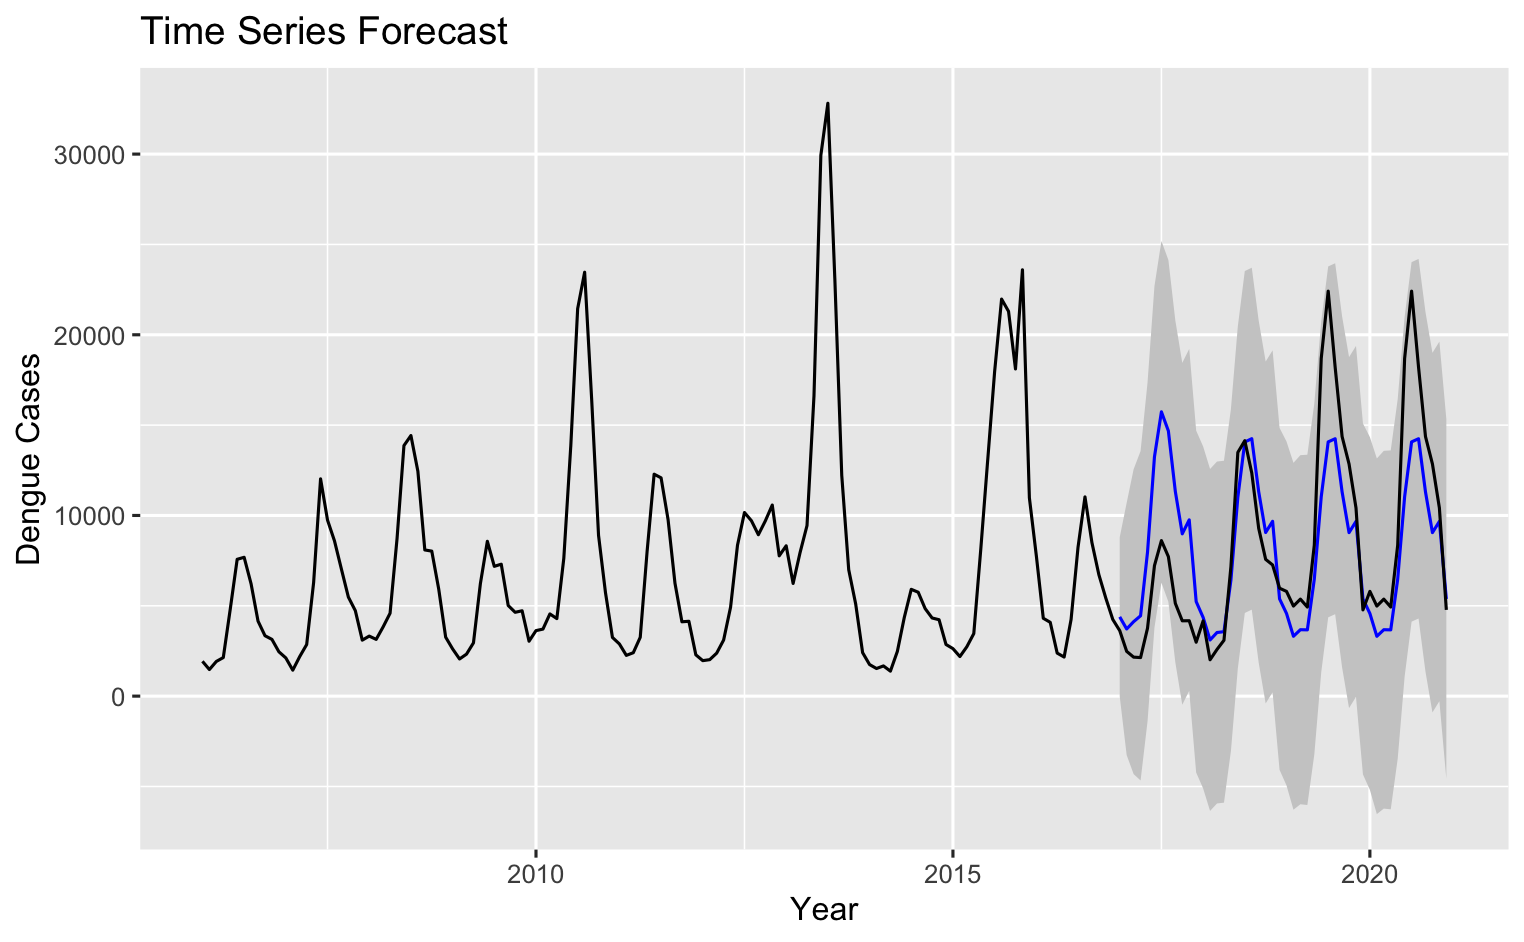
\includegraphics[width=0.7\textwidth]{fig/Auto_ARIMA_2016.png}
		\caption{ARIMA forecast of the dengue cases in Thailand for the years 2017-2020 (blue) compared to the actual dengue cases (black).}
		\label{fig:Auto_ARIMA_2016}
	\end{figure}

Although the forecast is more uniform than the actual cases in th years 2017 to 2020, the reported cases are in the range of deviation shown in grey. 

\subsection{GAM model}
A GAM model was generated based on the monthly temperature and incidence of all provinces of Thailand over the years 2006 - 2020. The predictor value (temperature) was passed into a smoothing function to create a smoothed spline curve. For the response variable (incidence) a quasi-Poisson distribution was chosen. The link function is a log transformation.
To figure out the optimal model, the degrees of freedom of the smoothing function were alternated. The effective degrees of freedom, which were found to be 13.82, resemble the complexity of the smooth curve. This value is relatively high, which indicates a “wigglier” spline. F-value and p-value indicate the statistical significance of the smooth function. In this case, the smooth function of temperature is highly significant (p-value < 2e-16). The computed R-squared value of 0.0465 indicates how well the model explains the variance in the dependent variable. Here, the model explains approximately 4,7\percent of the variance in the data. A low GCV (Generalized Cross Validation) value suggests a good fit of the model. The generated model has a GCV of 11.77. Additionally, the AIC value of the smooth model (112947.1) was compared with that of a linear model (113361.2). The smooth model had a lower value, which indicates a better fit.
Taking all these parameters into account, the GAM was computed with a k of 16. The model and its relationship of temperature and incidence is shown in the appendix Figure ..., as well as the evaluating graphs.
Subsequently the model was used to predict the average dengue case incidences over the period of 2021 until 2040, based on forecasted average temperature. You can see the average incidences of the past and future below.
